% !TeX document-id = {6d544fe2-4255-4108-8022-d809ff1d2c53}
% TeX program = xelatexmk %doesn't work, no xelatexmk option under 'build'. Changed default engine to xelatex (options-->configure-->build-->default build-->xelatex)
% see http://info.semprag.org/basics for a full description of this template
\documentclass[charis,linguex]{glossa}
% possible options: 
% [times] for Times font (default if no option is chosen)
% [cm] for Computer Modern font 
% [lucida] for Lucida font (not freely available)
% [brill] open type font, freely downloadable for non-commercial use from http://www.brill.com/about/brill-fonts; requires xetex
% [charis] for CharisSIL font, freely downloadable from http://software.sil.org/charis/
% for the Brill an CharisSIL fonts, you have to use the XeLatex typesetting engine (not pdfLatex)
% for headings, tables, captions, etc., Fira Sans is used: https://www.fontsquirrel.com/fonts/fira-sans
% [biblatex] for using biblatex (the default is natbib, do not load the natbib package in this file, it is loaded automatically via the document class glossa.cls)
% [linguex] loads the linguex example package
% !! a note on the use of linguex: in glossed examples, the third line of the example (the translation) needs to be prefixed with \glt. This is to allow a first line with the name of the language and the source of the example. See example (2) in the text for an illustration.
% !! a note on the use of bibtex: for PhD dissertations to typeset correctly in the references list, the Address field needs to contain the city (for US cities in the format "Santa Cruz, CA")

%\addbibresource{sample.bib} 
% the above line is for use with biblatex
% replace this by the name of your bib-file (extension .bib is required)
% comment out if you use natbib/bibtex

%for natbib: replace \cite with \citep (parenthetical); \citea with \cite (in-text)

\let\B\relax %to resolve a conflict in the definition of these commands between xyling and xunicode (the latter called by fontspec, called by charis)
\let\T\relax
\usepackage{xyling} %for trees; the use of xyling with the CharisSIL font produces poor results in the branches. This problem does not arise with the packages qtree or forest.
\usepackage[linguistics]{forest} %for nice trees!

\usepackage{tipa}
\newcommand{\nt}[1]{\textipa{[#1]}} % narrow transcription
\newcommand{\wt}[1]{\textipa{/#1/}} % wide transcription



%\graphicspath{{images/}}

% \pdf* commands provide metadata for the PDF output. ASCII characters only!
\pdfauthor{Auromita Mitra, Indranil Dutta}
\pdftitle{Mixed language processing increases cross-language phonetic transfer in Bengali-English Bilinguals}
\pdfkeywords{phonetic transfer, vowel formants, Bengali, English}

\title{Mixed language processing increases cross-language phonetic transfer in Bengali-English Bilinguals}
% Optional short title inside square brackets, for the running headers.


% \author[Auromita \& Indranil]% short form of the author names for the running header. If no short author is given, no authors print in the headers.
% {%as many authors as you like, each separated by \AND.
%   \spauthor{Auromita Mitra\\ 
%   \institute{The EFL University}\\
%   \small{%105, Bd. Raspail, 75005 Paris\\
%   auromita.mitra@gmail.com}
%   }
%   \AND
%   \spauthor{Indranil Dutta \\
%   \institute{Jadavpur University}\\
%   \small{%Warmoesberg 26, 1000 Brussel\\
%   indranildutta.lnl@jadavpuruniversity.in}
%   }%
% }
%\usepackage{gb4e}
\begin{document}

\sffamily
\maketitle

Word count: 6944

\begin{abstract}
Existing research demonstrates that mixed-language productions of bilingual speakers differ from productions in a single language. Studies have largely focused on temporal properties of consonants, and reported varied, and often contradictory, results. The present study examines the effect of mixed-language processing on two L2 vowel categories in a group of highly proficient Bengali-English bilingual speakers in India. Following from a discussion in \citep{olson2013bilingual}, we compare productions elicited in two paradigms-- cued picture-naming and code-switching. Results indicate a dynamic increase in cross-language phonetic transfer during mixed-language use leading to a shift towards L1 norms, asymmetrical shifts in the two categories, and no difference in transfer patterns between the two paradigms. 
\end{abstract}

\begin{keywords}
  
\end{keywords}

\rmfamily


\section{Phonetic transfer}

Bi/multilingual speakers can distinguish between the phonetic norms of their languages \cite{caramazza1973acquisition,macleod2010impact,bosch2003simultaneous} and therefore maintain separate sound categories for each language. However, these categories are not autonomous-- they show cross-language influence in both perception and production \cite{flege1995second,fowler2008cross,flege2002assessing}. What causes, affects, and results from such influence? Answers to these questions provide important insights into how language `systems' are represented and processed in the mind. %Given that a majority of the world's population is multilingual, this is a central concern for any realistic theory of language.
%show cross-language-- rephrase

%keep just the types here, and put the next 2 lines in the causes&effects section?
Cross-language influence at the level of sounds can be studied broadly in two kinds of conditions:
(i) While a bilingual speaker is operating in any one of their languages, by comparing bilingual speech to monolingual norms \citep[e.g.][]{guion2003vowel,caramazza1973acquisition,flege1987production}; %These studies often compare the speech of bilinguals to monolingual norms, and view the influence as changes to long-term memory representations as a result of acquiring an L2 \citep{guion2003vowel,caramazza1973acquisition,flege1987production}; 
(ii) When both languages of a bilingual speaker are co-activated, by comparing bilingual speakers' mixed-language speech to their own norms while using a single language \citep[e.g.][]{grosjean1994going, bullock2009trying,elias2017effects, simonet2014phonetic}. %These compare productions during mixed-language use to participants' own productions while using a single language. The resulting influence is variously thought to involve short-term memory, online processing costs, language mode, and context-awareness. 
The present study is concerned with the latter. In production, researchers have variously referred to this kind of influence as transfer, drift, accommodation, and interference-- these terms are used interchangeably here to indicate any interaction between two sets of phonetic norms.

Existing research on the phonetic effects of mixed-language production has largely focused on a few pairs of phonologically related languages. A majority of these studies use temporal properties of consonants (in particular, voice onset time or VOT) to measure transfer. However, the reported results vary greatly across studies, and appear to be contingent upon both language-specific features and language experience of the participants. This suggests that data from a wider variety of
%elaborate on 'great variation'-- differences between language pairs, plus sociolinguistic situation (effects of language experience etc)-- clearer. 'Types of features'--separate line?- Brief mention - discursive factors in VOT. 
populations, language pairs,  and phonetic features needs to be considered in order to make meaningful generalizations. There is no work yet on short-term phonetic transfer in the Indian subcontinent, or in any Indo-Aryan language. Nevertheless, widespread multilingualism in this part of the world suggests that phonetic
%line--rephrase
behavior in these populations can be particularly valuable towards understanding the nature of such cross-language interactions, as they are likely to reflect real-world experience with mixed-language processing.\\

The present study examines phonetic transfer between Bengali and English in a group of highly proficient bilingual speakers in India. We measure spectral properties (F1 and F2) of two English vowels to ascertain if L1 influence on L2 increases during mixed-language use, relative to a participant's unilingual baseline production of L2. Mixed-language data is elicited in two switching paradigms: code-switching and cued picture-naming. We compare these results to assess if differences between the paradigms independently influence the outcome of phonetic interaction. The results demonstrate a dynamic effect of transfer on L2 vowels during mixed-language production, but no difference in the extent of transfer between the two paradigms. Findings are discussed in light of recent proposals about asymmetries in short-term phonetic interaction and the role of connected speech in introducing discursive factors to transfer studies.\\


The rest of this section is structured as follows: \ref{bengali_english_in_india} provides background information on Bengali and Indian English focusing on vowel systems. \ref{causes} discusses two potential sources of transfer during language processing-- global co-activation of multiple languages vs the local act of switching between languages. Given the highly multilingual setting that characterizes this population, we note that the former is expected to be a constant feature and therefore any observed phonetic interaction is better understood as resulting from the latter. The design of the present study is motivated on the basis of this discussion. A logical consequence of this model is that such phonetic interaction must be highly localized. \ref{duration} elaborates on this by reviewing literature on the duration and `reversiblity' of transfer effects. A recurring pattern that emerges from existing research on short-term phonetic transfer is that the phonetic influence does not affect both languages of the bilingual speaker equally, although the nature of these reported differences varies greatly across studies. In \ref{asymmetries}, we review some of these findings, focusing on proposed sources of asymmetries, in order to highlight the factors that seem to mediate such phonetic interaction. We argue that these results point to an urgent need for expanding the range of language pairs and sound categories examined in order to make meaningful generalizations about the nature of short-term phonetic transfer. Following from this, \ref{asymmetry between sounds} discusses reported asymmetries between different sound categories of a single language, and develops the hypotheses of the present study on the basis of these. In \ref{paradigms}, we motivate a secondary aim of this study: to verify the postulated differences between two paradigms for eliciting short-term phonetic interaction in an experimental setup, namely code-switching and cued picture-naming. \ref{questions_and_hypotheses} summarizes the research questions and hypotheses.

\subsection{Bengali and English in India} \label{bengali_english_in_india}

\subsubsection{Demography} 

Bengali (also, Bangla) is an Indo-Aryan language primarily spoken in India and Bangladesh. In India, more than 97 million people speak Bengali as a first language (Census of India, 2011), mostly in the state of West Bengal. A majority of this population also speaks other additional languages.

Indian English (IE) refers to the variety of English that has developed in the Indian subcontinent. In India, it is spoken as an L2 by 129 million people (Census of India, 2011).  English is one of the two official languages, used in education, law, media, as a \emph{lingua franca} mainly for an educated elite in most metropolitan regions, and carries a high prestige value \citep{pandey201517, kachru1981english, tollefson2014language, kachru1983indianization}.
%citations 
Recent research comparing the segmental and suprasegmental properties of IE spoken in different parts of the country report many commonalities (see \cite{sirsa2013effects} for a review). This suggests that in spite of the varied L1s of its speakers, IE has a target phonology that is distinct from any of these, as well as from other native varieties of English. Thus, it is fruitful to think of regional variations as resulting from L1-influence on a common underlying target. Excepting a small minority of specific communities \citep{pandey201517, wells1982accents, coelho1997anglo}, there are very few L1 speakers of IE.\\

%%%%%%%%%%%%%%%%%%%%%%%do something%%%%%%%%%%%%%%%
Considering the language usage patterns suggested by this demography, the present study focuses on short-term phonetic interaction during mixed-language use, because:
\begin{enumerate}[label=(\roman*)]
	\item Since the population is multilingual, we expect long-term representations to be affected by multiple languages. 
	\item Given that examples of an IE phonology without L1 `influence' are very rare, it is more meaningful to think of cross-language transfer in L2 as relative to a speaker's own production in a given `baseline' condition.
\end{enumerate}

The socio-linguistic facts about English in India also suggest that for the present population, mixed-language processing of English and an L1 is an ecologically valid paradigm that is likely to be a part of everyday language experience. Thus, data from this population is valuable to the understanding of short-term phonetic interaction as it occurs in .

\subsubsection{Vowel systems} \label{vowel systems}
The vowel inventory of Western Bangla (the variety spoken by the participants in this study) consists of \nt{i, e, \ae, a, O, o, u}, and their nasalized counterparts \citep{garry2001facts}. Note that there is no mid-central vowel category. 


The vowel system of IE contains the monopthongs \nt{I, i, E, e, \ae, @/2, a:, O, o, U, u}, represented by the lexical set KIT, FLEECE, DRESS, FACE, and TRAP, STRUT, PALM, LOT/CLOTH, GOAT, FOOT, GOOSE \citep{wells1982accents, masica1972sound}. %Their distribution in the F1XF2 space is shown in (insert table 1.7, Pandey). 
A single mid-central vowel corresponds to the categories \nt{2,@,3:}, which are treated as distinct in many native varieties of English \citep{nihalani1979indian,wells1982accents,hickey2005legacies,bansal1969intelligibility}. Since the English items used in this study are traditionally transcribed with \nt{2}, we use this symbol to indicate the mid-central vowel throughout. 
 

\subsection{What causes transfer and what does it affect?}\label{causes}

Existing research has distinguished changes in category \textsc{representations} due to the acquisition of multiple sound systems (cf. Speech Learning Model \citep{flege1995second,flege2007language}; Perceptual Assimilation Model-L2 \citep{best2007nonnative}), from interaction during accessing, processing, or articulation of these categories (cf. transfer vs interference \citep{grosjean2012attempt}; competence vs performance interference \citep{paradis1993linguistic}). 
Given their transient nature, dynamic changes in production during mixed-language use are generally attributed to the latter, e.g. online processing costs \citep{olson2013bilingual,tsui2019impact,vsimavckova2015immediate}, language mode \cite{simonet2014phonetic}, context-awareness \citep{khattab2013phonetic}. What triggers this interaction? \cite{olson2016role} argues that while cross-language phonetic effects are largely measured at the point of language switch, it could have two potential sources:
\begin{enumerate}
	\item The local point of switch itself
	\item Global co-activation of two languages -- bilingual language mode \citep{grosjean1998studying} 
\end{enumerate}

A number of studies have specifically manipulated language mode, both in the presence and absence of switching. Overall, results suggest that (i) In the absence of other manipulations, productions in a bilingual language mode show increased cross-language influence compared to a monolingual mode \citep{simonet2020increased,simonet2014phonetic}; (ii) However, language mode is not the sole source of influence during mixed language use -- studies comparing switched and non-switched tokens produced in the same test block (identical language mode) \citep{olson2016role,tsui2019impact} or spontaneous conversation \citep{piccinini2015voice}, have still reported a difference, suggesting that independently of mode, switching between languages triggers a local increase in cross-language transfer. (iii) How the two sources interact to influence the final outcome of transfer is not fully understood-- \cite{olson2016role} found no additive effects, \cite{olson2013bilingual} found the balanced language context to inhibit transfer compared to unbalanced contexts.  Other studies have not analyzed the two separately, eliciting switched tokens in a bilingual test block and non-switched tokens in a separate monolingual test block, separated by a few hours to days \cite{Pschwartz2015language, bullock2009trying,antoniou2011inter, elias2017effects,vsimavckova2015immediate,vsimavckova2018patterns}.

\cite{grosjean1998studying} suggests that various aspects of the communicative setting, including exposure to (spoken or written) stimuli in multiple languages and awareness of the interlocutor's being bilingual, could trigger a bilingual mode. The participants in the present study are in an environment which largely contains mixed-language input, multilingual interlocutors, and no stable ambient language. Therefore we expect that phonetic transfer during everyday language use, if any, takes place in a bilingual mode.  To preserve ecological validity, we elicited both unilingual and switched utterances in a bilingual language mode. Any observed differences in this paradigm would arguably result from interaction during online processing. 

In a bilingual mode, both language systems are expected to be (nearly) equally accessible throughout the test block. Thus, a consistent difference between switched and non-switched tokens in such a paradigm would be possible only if the effects were highly localized (if not, we should expect a gradual convergence over the course of the experiment). This is discussed in the next section.

\subsection{Duration: How long do effects last?} \label{duration}

Studies which compare bilinguals speakers' phonological systems with monolinguals see them as relatively stable over time. The difference from monolingual norms is interpreted as the cumulative result of cross-language influence over long periods, \cite{guion2003vowel, caramazza1973acquisition}. However, longitudinal studies %(citations) 
and between-subject comparisons of bilingual speakers who differ in the duration of L2 exposure suggest that interaction between the sound systems is dynamic. Over time, increasing exposure to an L2 can reduce effects of L1 influence, leading to a more fine-grained separation and native-like production of foreign contrasts-- e.g. \cite{bohn1992production} 
found that an approximately 7 years' difference in L2 exposure between groups having the same age of acquisition led to a significant difference in the amount of cross-language transfer. These have been interpreted as changes to long-term phonological representations.

Moreover, changes due to transfer are not unidirectional or irreversible. \cite{sancier1997gestural} first demonstrated that spending 2-5 months in an L1 or L2 environment causes productions in both languages to ``drift" towards the ambient language. This not only showed that cross-language interaction can be triggered in an order of months, but also that the effects can be reversed within a similar time range. A recent study by \cite{tobin2017phonetic} found comparable effects in an even shorter duration (2-4 weeks). A short-term longitudinal study by \cite{chang2012rapid} showed that over the course of the first five weeks of learning an L2, there was a gradual convergence of L1 towards L2. For some sounds and features (though not others, cf sec.\ref{asymmetry between sounds}), transfer was additive over time. How long these effects last in the absence of regular L2 input was not tested. 
% if effects are cumulative, then the difference between switched and non-switched tokes should be lesser in later test blocks (previous two paragraphs needed?)

Studies examining mixed-language use within an utterance mostly analyze only the switched (target) token. Thus, very few direct measurements of the duration of transfer effects are available. One study which measured this \citep{bullock2009trying} did not find any residual effects on the matrix language following a switch, suggesting that transfer during code-switching is localized.  

More indirect evidence for this comes from studies which have elicited switched and non-switched tokens in the same test block \citep{tsui2019impact,olson2013bilingual}, and still reported differences between the two, suggesting that changes due to transfer are quickly `reset'-- in an order of seconds. Note that all these studies measure VOT, which is a temporal feature. We have no apriori reason to assume that these durations generalize to vowel quality. However, findings from sub-categorical phonetic shifts triggered by other factors (such as convergence towards an interlocutor) do evidence rapid shifts in vowel quality within comparable time-frames \citep{pardo2010expressing,babel2010dialect,babel2012evidence}. Thus in the current study, we present switched and non-switched tokens randomly within the same test block to induce a bilingual mode. We expect the intervening words between two subsequent targets to undo any residual effects of transfer.


\subsection{Asymmetries between languages in extent and direction of transfer} \label{asymmetries}
Previous research has largely reported asymmetrical shifts between languages. Two proposed sources of such differences that are relevant to this study are discussed below: 

\subsubsection{L1 vs L2 status} 
Flege's Speech Learning Model (SLM) \citeyear{flege1995second,flege2007language} posits that the sound categories of a bilingual speaker exist in a common phonological space, and thus in principle, both L1 and L2 sounds can affect one another. Thus, the patterns of cross-language transfer depend on the mapping of L2 phonemes in relation to existing L1 categories. In non-switched production, this is evidenced through a pervasive L1 influence on non-native contrasts that are perceptually linked to an existing L1 contrast (equivalence classification-- \cite{flege1984limits,flege1987production}), and
the observation that both the L1 and L2 sound systems of bilinguals differ from corresponding monolingual speakers \citep{guion2003vowel}. 

In mixed-language production, the role of language status is less clear-- studies have reported unidirectional influence of L1 on L2 \citep{balukas2015spanish,antoniou2011inter,vsimavckova2015immediate,goldrick2014language}, L2 on L1 \citep{tsui2019impact,elias2017effects, olson2013bilingual}, bidirectional convergence \citep{bullock2009trying, olson2016role}, divergence \citep{bullock2009trying,vsimavckova2018patterns}, and no influence \citep{muldner2019phonetics,schwartz2015language}. Since most existing studies measure shifts in VOT, the observed asymmetries between languages have been variously explained either in terms of their L1 vs L2 status, or language-specific differences between long- and short-lag VOT languages (cf sec. \ref{sound systems}).

\cite{olson2013bilingual} first reported a unidirectional VOT shift of L1 towards L2 in two different groups -- native speakers of Spanish (short-lag) and English (long-lag), matched for proficiency and age of L2 acquisition. This suggested that beyond language-specific differences, the L1 vs L2 status of the language does mediate transfer. They explain the asymmetry in terms of the Inhibitory Control Model (ICM) \citep{green1998mental} -- to select a phonetic realization from one language, the other must be inhibited. Being the `stronger' language, more inhibition is required on the L1. Thus, switching into L1 incurs a greater switch-cost (more cross-language influence) than switching into L2. The lesser switch cost results in a lack of visible cross-language transfer effects on L2. \cite{tsui2019impact} found comparable results, but only in participants who were not equally dominant in both languages. Balanced bilinguals did not demonstrate any transfer effects in VOT. They propose that this is because balanced bilinguals have better inhibitory control (low switch costs in both languages) due to greater experience with language switching.

Since VOT is independently affected by short- vs long-lag differences, studies of other sound contrasts/features can avoid this conflation, and give a clearer picture of the effect of language status. However, given the implications of the ICM, we would first have to establish that these L2 categories can indeed be affected by dynamic interference. The few existing studies which focus on vowel quality \citep{simonet2014phonetic,muldner2019phonetics,elias2017effects} and phonological processes \citep{simonet2020increased,schwartz2015language} have all examined transfer effects on L1. As far as we are aware, there has been no work yet on vowels in L2. Thus, this study builds on the existing work by examining whether the L2 vowel quality of proficient bilinguals can be affected by mixed-language processing.

\subsubsection{Differences between sound systems of the languages} \label{sound systems} In addition to the cognitive factors discussed above, many studies have attributed the asymmetries to language-internal factors. Specifically, a pattern that emerges from the body of work on VOT is that a shift in long-lag VOT towards the short-lag norms of the other language is much more consistent and systematic than the converse \cite{tobin2017phonetic, olson2016role,bullock2009trying,antoniou2011inter,chang2012rapid}. In general, short-lag VOTs seem to resist accommodative shift. \cite{bullock2009trying} suggest that because long-lag languages offer a greater range of acceptable VOTs, there is more `room' for movement. In contrast, shift in short-lag languages could risk the loss of a phonological contrast (VOT being the primary cue for voicing contrast in these languages).  This is a language-specific phonological constraint on transfer.
In a similar vein, \cite{antoniou2011inter} found that while English stops shifted towards Greek (a short-lag language), the reverse was seen only in a subset of sounds-- word-medial non-nasalized stops. They attribute this to the low frequency of these sounds in Greek, which makes them less `stable', and thus more amenable to shift. This suggests that the distribution of sounds in a language could affect the kind of transfer patterns observed.

These results highlight that beyond interaction during the cognitive processing of sounds, phonetic transfer is ultimately a linguistic phenomenon, and thus subject to language-specific phonological constraints. Therefore, to make meaningful generalizations, it is imperative to consider data from a variety of language pairs. Existing research on phonetic transfer largely revolves around a small set of phonologically related languages. Thus, the present study extends the scope of this research to a new set of languages---Indian English and Bengali (an Indo-Aryan language).

Since Bengali has a four-way laryngeal contrast, VOT does not encode a binary voiced---voiceless distinction, and moreover is not the only cue for the corresponding phonological categories \citep{dmitrieva2020acoustic}. Thus, the effects of Bengali on English VOT are likely to be affected by additional phonological factors. Thus, avoiding any potential confounds was another reason we chose to focus on vowels as a target for transfer. 


\subsection{Asymmetries between sounds}\label{asymmetry between sounds}

Existing research reports asymmetrical transfer effects not only between languages, but also between different sounds/features in a language, in both long-term and transient interactions. Studies which have examined multiple sound categories have found that interactions between individual sounds pairs do not necessarily reflect the overall pattern of global (system-wide) shift \citep{chang2012rapid,elias2017effects}, suggesting that `extent of transfer' cannot be seen as an atomic measure. In light of the discussion in section \ref{sound systems}, this is not surprising -- if a general linguistic principle of `room for movement' constrains transfer, then we should expect it to apply to individual sounds too. Once again, this emphasizes the need to study a wider range of sound contrasts.


In the present study, we examine two vowel categories in Indian English-- the mid-central vowel \nt{2} and the low front vowel \nt{\ae}. There are two plausible sources of asymmetry between these:
\begin{enumerate}
	\item Position in the vowel space of IE: \nt{2} is in a less crowded part of the vowel space, and thus has more latitude for movement without risking contrast, particularly in the height (F1) dimension. Thus, considering purely phonological constraints on IE, we would expect that a greater degree of shift is possible in \nt{2} compared to \nt{\ae}. Any movement in \nt{\ae} is expected to be primarily in the front-back (F2) dimension.
	\item Target of transfer: Since we do not elicit unilingual L1 utterances in this study, we cannot directly compare the target vowels to baseline L1 vowels. However, the body of existing research on phonetic transfer suggests that shifts are targeted with respect to categories in the other language, rather than random. Thus, another source of asymmetry is the fact that \nt{2} is not present as a phoneme in Bengali, whereas \nt{\ae} is a common category across both languages (cf sec.\ref{vowel systems}).
\end{enumerate}

%table

Flege's Speech Learning Model (SLM) \citep{flege1995second,flege2007language} suggests that sound categories which are common across languages influence each other because they share a common acoustic-phonetic space. Thus, if Bengali and English differ in their canonical realizations of \nt{\ae}, then we should expect the English \nt{\ae} to shift towards the corresponding Bengali category in the mixed condition. 

%Other categories can in principle be produced with native-like accuracy, showing little effect of transfer. Given that our participants are highly proficient bilinguals, and assuming that cross-language correspondences remain the same in representation and processing, this would lead us to expect more transfer in the common category, \nt{\ae}. 

There is no obvious competing L1 category during the production of \nt{2}. However, it is unlikely that this should altogether preclude a shift in \nt{2}, since at least one existing study has reported transfer effects on a non-common vowel category in a comparable paradigm \citep{simonet2014phonetic}. Here, the Catalan \nt{O} moved towards an acoustically close category \nt{o}, which is common to Catalan and Spanish, suggesting that shift might be towards a set of phonetic norms rather than a particular target. 

The vowel \nt{2} is thus expected to shift towards an acoustically close category in IE -- a probable candidate being the low vowel \nt{a:}, as anecdotal observations of heavily-accented English suggest that the sounds are perceived as close by Bengali speakers. 

As noted above, we did not elicit unilingual Bengali productions from the participants in this study. To estimate a baseline value for the relevant Bengali vowels, productions in the unilingual English condition were compared to data from five female Bengali speakers from \cite{dutta2016using}. Formant values were extracted from syllable-initial productions of \nt{\ae} and \nt{a:}, at 55\% into the vowel. Comparisons of Lobanov-normalized F1 and F2 suggests that the Bengali category \nt{\ae} is lower, and \nt{a:} lower and more fronted, compared to the English categories \nt{\ae} and \nt{2} respectively. 

\subsection{A note on paradigms: connected speech or not?} \label{paradigms}

Studies of phonetic transfer during mixed-language use have largely used spontaneous or scripted code-switching (CS, defined as the use of multiple languages within a single utterance, ie in connected speech; \citealp{myers1993dueling}) to co-activate the two languages. Other paradigms include cued picture-naming, delayed repetition, interpreting across languages, reading word-lists etc. \cite{olson2013bilingual} argues that code-switching introduces discursive factors such as discourse planning and pragmatic considerations, which ultimately show patterns of language practice, rather than cognitive behavior. This finds support from studies which report transfer effects before the switch point \citep{bullock2009trying}, or other evidence of planning such as hyperarticulation \citep{muldner2019phonetics} and interlocutor-awareness in spontaneous CS \citep{khattab2013phonetic}. To avoid such confounds, Olson suggests cued picture-naming (where pictures are named in rapid succession in either language, based on the given language cue) as an alternative paradigm to isolate purely phonetic effects in controlled setups. 

Note that while there is evidence for planning in CS, exactly how this affects phonetic transfer cannot be predicted from the existing literature-- while \citep{bullock2009trying} found tokens immediately preceding the switch point to be phonetically distinct from the rest, one group showed convergence towards the switch language(explained in terms of proficiency) while the other showed divergence (explained in terms of extra-linguistic factors). The participants in Muldner et al.'s \citeyear{muldner2019phonetics} study hyperarticulated switched tokens (suggesting some degree of planning), and showed no significant shift. Moreover, recall that Olson's \citeyear{olson2016role} findings suggest that there is a limit on transfer-- multiple factors do not necessarily lead to additive effects. Thus, the existence of additional factors in CS does not automatically mean that this should affect the extent of transfer compared to any other paradigm. It is possible that the effects in the studies mentioned above could be attributed to some other aspect of the experimental setup, rather than a result of code-switching in particular.

While much more work is necessary to tease out the various factors and their interactions, the focus of the present study is to check whether, in an experimental setting, the postulated discursive elements in a CS paradigm affect the extent of observed transfer, compared to a paradigm which arguably lacks them--cued picture-naming. We are less concerned with the exact nature of differences, than with their comparability. While studies using each of these paradigms to induce transfer exist, comparison across studies is difficult, since they also differ in other factors. This study thus provides a starting point for such comparison by eliciting productions of the same tokens from the same participants, in both paradigms. A difference in the extent of transfer will suggest that the planning effects in connected speech affect transfer independently of the phonetic results of switching, which has implications that future studies should look into. 


\subsection{Research questions and hypotheses}\label{questions_and_hypotheses}
\begin{itemize}
	\item Are L2 vowel categories of proficient bilingual speakers affected by dynamic phonetic transfer during mixed-language production?
	\item If so, we expect an asymmetry between the vowels in the extent and direction of shift. Based on comparisons with Bengali vowels from \cite{dutta2016using} we expect \nt{2} to be lowered and fronted in the mixed condition. \nt{\ae} is expected to show lowering, but to a lesser extent than \nt{2}, as it is in a part of the IE vowel space that has greater vowel density.
	\item Is there an observable difference in the extent of transfer between the cued picture-naming and the code-switching paradigms? 
\end{itemize}


\section{Methodology} \label{methodology}
The experiment had the following factorial design: 10 participants*20 target words*2 conditions *2 tasks *4 iterations = 3200 target items

\subsection{Participants}

10 Bengali-English bilingual speakers (male=5, age range 19 to 28), completed the tasks. All the participants speak other languages in addition to Bengali and English. At the time of recording, they were living in or around the EFL University campus in Hyderabad, which has a linguistically diverse population. Speakers were selected on the basis of responses to a Language Background Questionnaire to ensure comparable LSRW skills in L1 and L2 across participants, and were compensated for their time.


\subsection{Stimuli}
Twenty monosyllabic English words containing the vowels \nt{2} or \nt{ae} were selected as target words. To minimize coarticulatory effects on the vowel, the pre-vocalic consonants were all voiced plosives (\nt{b} or \nt{d}). 10 monosyllabic English words that do not contain the target vowel served as filler items. English words which are lexicalized loanwords in Bengali were avoided. %The list of words can be found in sec.\ref{appendix}.



\subsection{Procedure}
Participants were recorded individually in a sound attenuated room. %, using a ... microphone type/description?
Productions were recorded in Praat \citep{boersma2016praat} at a 44.1K sampling rate. Every participant performed four iterations each of two tasks-- cued picture-naming and code-switching. Utterances in the two conditions (unilingual and mixed) were randomly interspersed within each iteration. In the unilingual condition, the target word was preceded by another English word in the utterance, whereas in the mixed condition, the target was produced as a switch from Bengali. Every target word appeared twice during a test block; once in a unilingual and once in a mixed condition. Participants alternated between the two tasks, and were allowed to take a short break after each test block.

The tasks are described below:


\begin{enumerate}[]
	\item Cued picture-naming: Participants were presented with slides in the following sequence-
	\begin{itemize}
		\item Language cue- a word in either English or Bengali orthography
		\item A picture displayed for 50ms; named by the participant in either English or Bengali, depending on the language cue 
		\item Target -- an English word; read out by the participant
		\item Distracter math problem
	\end{itemize}
	Since all the target words were in English, the language cue was used to manipulate the preceding word, giving target words in non-switched (unilingual) and switched (mixed) utterances. The orthographies of English and Bengali are visually distinct, and were thus used to cue language.
	
	\item Code-switching: Each slide contained one target word embedded in either an English (unilingual) or a Bengali (mixed; target produced as a switch from Bengali) carrier sentence which was read out by the participant. The carrier sentences are given below:
	\begin{itemize}
		\item Unilingual sentence: That is a yellow [Target Word].
		\item Mixed-language sentence: \textipa{o-\:ta \ae k-\:ta kalo} [Target Word]. 
	\end{itemize}
	
Gloss and translation for Bengali sentence:

	o-ta \quad Ek-ta \quad kalo [target word]\\
	that-CL one-CL black [target word]\\
	that is a black [target word]\\

	The sound preceding the target word was uniform across all sentences (the final sound in `yellow' is produced as [o] in Indian English), to minimize any possible differences due to coarticulatory effects on the target word. A specifier-noun construction was used to ensure identical word order in both languages, giving uniform prosodic context for the target word. Mixed orthography was used for the mixed-language utterances. \\
	
\end{enumerate}
\subsection{Acoustic analysis}\label{analysis}
The first iteration of each task was treated as a trial, and excluded from analysis. An additional 67 tokens (2.79\%) were excluded due to errors in presentation/production, giving 2333 target word items for analysis. Recordings were manually segmented and annotated in Praat \citep{boersma2016praat}, and the first and second formant frequencies (F1 and F2) of the target vowels \nt{2, ae} were measured at five points-- in 10\% increments starting at 5\% into the vowel. This gave measures of F1 and F2 at 5\%, 15\%, 25\%, 35\% and 45\% into the vowel, allowing us to observe any dynamic changes in the extent of transfer over the course of producing the vowel.


\section{Results} \label{results}

%Figures ... show the findings of the experiment. 
All statistical analyses were performed in R \citep{r}. The dependent variables were vowel height (F1) and backness (F2). We fitted a series of linear mixed effects models using the \emph{lme4} package \citep{lme4}, to examine the effect of experimental conditions on lobanov normalized F1 and F2 at each of the five points in the vowel (sec.\ref{analysis}). For all mixed models, the alpha criterion was set at $|t| > 2 $. The independent variables or fixed factors, along with their levels, are given in table \ref{table variables}. Subject and Item were treated as random factors.

\begin{table}
	\caption{Fixed factors}
	\sffamily
	\centering
	\begin{tabular}{p{0.5\textwidth}p{0.5\textwidth}}
		\hline 
		Factor & Levels\\ 
		\hline
		Gender & male, female\\
		Vowel & \nt{2}, \nt{\ae} \\
		Task (corresponding to the two paradigms) & p (Picture: cued picture-naming, s (Sentence: code-switching)\\
		Context (corresponding to the experimental conditions) & e (English: unilingual), b (Bengali: mixed)\\ [1ex]
		\hline	
	\end{tabular}
	\label{table variables}
\end{table}



Since we wanted to model height and backness at different points in the vowel using a single model, allowing us to track if/how transfer changes over time, we arbitrarily chose a point in the vowel (F1 at 25\%; henceforth $F1\_25$) to identify an optimal model, and then fitted this to all other points. 

Vowel quality and gender are expected to systematically affect F1. Thus, we began with a model that had Vowel and Gender as fixed effects, random intercepts for Subject and Item, and random slopes for each within-unit variable that was relevant to our hypotheses-- by-subject slopes for Task, Context, and Vowel; by-item slopes for Task and Context. Next, adding Context as a fixed effect significantly improved the model fit ($\chi^2(1) = 5.54, p= 0.01854$), suggesting that the experimental condition affects vowel height. However, since we expected the extent of change in vowel height between the conditions to depend on the identity of the vowel (cf sec.\ref{asymmetries}), we added a two-way interaction factor between Vowel and Context. As expected, this was found to significantly improve model fit ($\chi^2(1) = 12.61, p= 0.0003837$). To check if the experimental paradigm affected F1, we added Task as a fixed effect, and this marginally improved the model ($\chi^2(1) = 3.74, p= 0.05302$). Following from the hypothesis in sec.\ref{paradigms}, we expected the extent of shift to differ across the two paradigms. However, no significant improvement was achieved by adding an interaction effect between Task and Context. Subsequent additions of other interactions, and removing each of the fixed effects in turn, did not lead to any further improvement. 

Context and Vowel are both within-subject factors. Since our hypothesis concerns their interaction, we modified the random effects structure by adding a by-subject random slope for the interaction term \citep{brauer2018linear}. This improved the model fit ($\chi^2(5) = 11.43, p = 0.04342$). Thus, we report on the model including Gender, Task, Context, Vowel, and a Context-Vowel interaction as fixed effects, random intercepts for Subject and Item, by-subject random slopes for Task, Context, Vowel and the Context-Vowel interaction, and by-item random slopes for Task and Context.

The following sections discuss the results for vowel height and backness respectively:

\subsection{Vowel Height -- F1}

Table \ref{table_f1_fixed_effects} summarizes the results of the fixed effects from the model for F1 at each point. As expected, we observe a significant effect of gender, such that male speakers have a lower mean F1 than female speakers. Vowel is not a significant predictor of F1. This seems surprising, given that the phonemic category is expected to systematically affect vowel quality. However, a boxplot visualization (Figure\ref{boxplot_F1}) shows that the participants in this study vary greatly both in the relative heights of the two categories and the extent of height difference between them. Note that these measures are only from the English (unilingual) condition, suggesting that the variability is a feature of the participants' IE vowel categories, independent of the effects of switching. The lack of any independent effect of Context on F1 suggests that using English words in mixed utterances does not lead to a uniform lowering/raising across vowels. Instead, the significant interaction between Context and Vowel indicates a lowering in \nt{2}, but not in \nt{\ae}, in the mixed-language condition. The results also reveal a significant effect of Task, such that the sentence task (code-switching) leads to higher F1 values in both vowels, relative to the cued picture-naming task. This effect is strongest at the beginning of the vowel, and disappears by 45\%. This is an unexpected result, since we have no principled reason to expect code-switching to induce an across-board lowering of vowels. As noted earlier, there is no significant interaction of Task with any of the other fixed factors. We used a series of ANOVAs to compare the above model with a null model that differs in the absence of the main factor which concerns our hypothesis-- Vowel*Context-- at each point in the vowel. We find that the effect is not significant at 5\%, and increases over the course of articulating the vowel. 
%ANOVA table add


\begin{figure}
	
	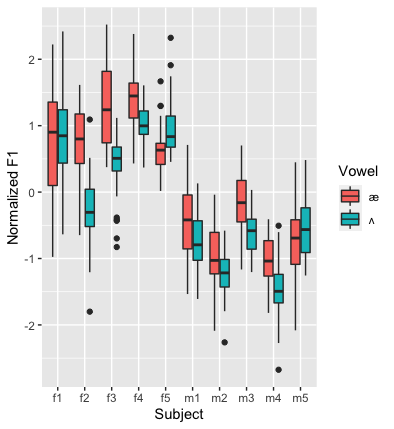
\includegraphics[scale=0.8]{vowel_by_subject_ggplot}
	\caption{Subject-wise mean F1; unilingual English}
	\label{boxplot_F1}
\end{figure}



\begin{table}[htbp] \centering 
	\caption{Model outputs for F1 at each of the five points in the vowel} 
	\label{table_f1_fixed_effects} 
	\begin{tabular}{@{\extracolsep{5pt}}lccccc} 
		\\[-1.8ex]\hline 
		\hline \\[-1.8ex] 
		& \multicolumn{5}{c}{\textit{Dependent variable:}} \\ 
		\cline{2-6} 
		\\[-1.8ex] & F1\_5 & F1\_15 & F1\_25 & F1\_35 & F1\_45 \\ 
		\\[-1.8ex] & (Model 1) & (Model 2) & (Model 3) & (Model 4) & (Model 5)\\ 
		\hline \\[-1.8ex] 
		(Intercept) & 0.447$^{**}$ & 0.718$^{***}$ & 0.750$^{***}$ & 0.863$^{***}$ & 0.921$^{***}$ \\ 
		& (0.211) & (0.176) & (0.153) & (0.152) & (0.150) \\ 
		& & & & & \\ 
		Gendermale & $-$1.171$^{***}$ & $-$1.526$^{***}$ & $-$1.586$^{***}$ & $-$1.668$^{***}$ & $-$1.681$^{***}$ \\ 
		& (0.237) & (0.184) & (0.168) & (0.177) & (0.175) \\ 
		& & & & & \\ 
		Contexte & $-$0.010 & $-$0.015 & 0.033 & 0.025 & 0.037 \\ 
		& (0.058) & (0.057) & (0.042) & (0.040) & (0.035) \\ 
		& & & & & \\ 
		Vowel\nt{2} & 0.022 & $-$0.070 & $-$0.034 & $-$0.131 & $-$0.216 \\ 
		& (0.170) & (0.175) & (0.170) & (0.174) & (0.168) \\ 
		& & & & & \\ 
		Tasks & 0.319$^{***}$ & 0.235$^{***}$ & 0.172$^{**}$ & 0.133$^{*}$ & 0.102 \\ 
		& (0.091) & (0.083) & (0.081) & (0.077) & (0.073) \\ 
		& & & & & \\ 
		Contexte:Vowel\nt{2} & $-$0.126$^{**}$ & $-$0.138$^{**}$ & $-$0.185$^{***}$ & $-$0.191$^{***}$ & $-$0.192$^{***}$ \\ 
		& (0.056) & (0.060) & (0.055) & (0.064) & (0.066) \\ 
		& & & & & \\ 
		\hline \\[-1.8ex] 
		Observations & 2,333 & 2,333 & 2,333 & 2,333 & 2,333 \\ 
		Log Likelihood & $-$1,771.558 & $-$1,589.316 & $-$1,278.310 & $-$1,313.795 & $-$1,380.083 \\ 
		Akaike Inf. Crit. & 3,599.116 & 3,234.631 & 2,612.621 & 2,683.589 & 2,816.165 \\ 
		Bayesian Inf. Crit. & 3,760.253 & 3,395.769 & 2,773.758 & 2,844.727 & 2,977.303 \\ 
		\hline 
		\hline \\[-1.8ex] 
		\textit{Note:}  & \multicolumn{5}{r}{$^{*}$p$<$0.1; $^{**}$p$<$0.05; $^{***}$p$<$0.01} \\ 
	\end{tabular} 
\end{table} 


\subsection{Vowel backness -- F2}

Table \ref{table_F2_fixed_effects} summarizes the results of fixed effects from the model for F2 at each point. Once again, we see that male speakers have a lower mean F2 than female speakers, as expected. The estimates for Vowel show that excepting the beginning of the vowel, the category \nt{2} is consistently produced as more backed than \nt{\ae}. Unlike vowel height, Context has an independent effect on vowel backness, such that both the vowels in this study have lower F2 values in the English (unilingual) condition, i.e. they are fronted in the mixed condition. A significant interaction between Vowel and Context shows that there is a difference in the extent of fronting between the two vowels -- the shift is greater in the case of \nt{\ae}. We see a significant effect of Task on F2, such that vowels in the sentence task (code-switching) were more backed than those in the picture-naming task. As with F1, this is an unexpected result. A lack of significant interaction with Context suggests that there is no difference in the extent of shift between the two paradigms. The results of ANOVAs comparing the full model to a null model which lacks the Vowel*Context interaction factor show that as with vowel height, the change in vowel backness between the two conditions is not significant at 5\%, and increases over the course of the vowel.

\begin{table}[htbp] \centering 
	\caption{Model outputs for F2 at each of the five points in the vowel} 
	\label{table_F2_fixed_effects} 
	\begin{tabular}{@{\extracolsep{5pt}}lccccc} 
		\\[-1.8ex]\hline 
		\hline \\[-1.8ex] 
		& \multicolumn{5}{c}{\textit{Dependent variable:}} \\ 
		\cline{2-6} 
		\\[-1.8ex] & F2\_5 & F2\_15 & F2\_25 & F2\_35 & F2\_45 \\ 
		\\[-1.8ex] & (Model 1) & (Model 2) & (Model 3) & (Model 4) & (Model 5)\\ 
		\hline \\[-1.8ex] 
		(Intercept) & 0.607$^{***}$ & 0.838$^{***}$ & 0.778$^{***}$ & 0.827$^{***}$ & 0.826$^{***}$ \\ 
		& (0.222) & (0.213) & (0.211) & (0.203) & (0.204) \\ 
		& & & & & \\ 
		Gendermale & $-$0.839$^{***}$ & $-$0.891$^{***}$ & $-$0.807$^{***}$ & $-$0.750$^{***}$ & $-$0.748$^{***}$ \\ 
		& (0.124) & (0.106) & (0.107) & (0.116) & (0.109) \\ 
		& & & & & \\ 
		Contexte & 0.003 & $-$0.088$^{**}$ & $-$0.065$^{**}$ & $-$0.063 & $-$0.103$^{***}$ \\ 
		& (0.036) & (0.036) & (0.032) & (0.044) & (0.033) \\ 
		& & & & & \\ 
		Vowel\nt{2} & $-$0.217 & $-$0.615$^{***}$ & $-$0.651$^{***}$ & $-$0.801$^{***}$ & $-$0.836$^{***}$ \\ 
		& (0.175) & (0.183) & (0.175) & (0.168) & (0.166) \\ 
		& & & & & \\
		Tasks & $-$0.234$^{***}$ & $-$0.194$^{***}$ & $-$0.152$^{***}$ & $-$0.141$^{***}$ & $-$0.092$^{**}$ \\ 
		& (0.029) & (0.035) & (0.050) & (0.047) & (0.045) \\ 
		& & & & & \\
		Contexte:Vowel\nt{2} & 0.031 & 0.110$^{***}$ & 0.128$^{***}$ & 0.091$^{**}$ & 0.147$^{***}$ \\ 
		& (0.050) & (0.041) & (0.040) & (0.046) & (0.043) \\ 
		& & & & & \\   
		\hline \\[-1.8ex] 
		Observations & 2,333 & 2,333 & 2,333 & 2,333 & 2,333 \\ 
		Log Likelihood & $-$1,283.531 & $-$1,478.494 & $-$1,174.087 & $-$1,222.682 & $-$1,019.033 \\ 
		Akaike Inf. Crit. & 2,623.062 & 3,012.988 & 2,404.175 & 2,501.363 & 2,094.066 \\ 
		Bayesian Inf. Crit. & 2,784.199 & 3,174.125 & 2,565.312 & 2,662.501 & 2,255.204 \\ 
		\hline 
		\hline \\[-1.8ex] 
		\textit{Note:}  & \multicolumn{5}{r}{$^{*}$p$<$0.1; $^{**}$p$<$0.05; $^{***}$p$<$0.01} \\ 
	\end{tabular} 
\end{table} 




\section{Discussion and Conclusion}

With regard to our first research question, the results confirm that the L2 vowels of proficient bilinguals can be affected by mixed-language processing. Both vowels in this study showed systematic shifts in the mixed-language condition compared to baseline unilingual productions. This is significant in the context of an ICM-based analysis of between-language asymmetries in phonetic transfer as proposed by \citep{olson2013bilingual}, because it demonstrates that at least for vowels, the postulated lower switch cost on an L2 does not entirely mask transfer effects. Thus, following from the discussion in sec. \ref{asymmetries}, it might be fruitful for future studies to focus on vowels as a site for transfer. This would both expand the scope of the existing research (cf sec. \ref{asymmetry between sounds}) and avoid confounding factors arising from independent differences between long- and short-lag VOT languages.

We hypothesized an asymmetrical shift between the two vowels, owing to differences in (i) their positions in the Indian English vowel space, and (ii) the existence of a corresponding category in the L1 Bengali inventory. The significant interaction between Vowel and Context in both F1 and F2 confirm that the experimental condition affected both height and backness differently for each vowel. As expected, we find a greater degree of shift in \nt{2}, possibly owing to its position in a less crowded part of the IE vowel space.
Figure \ref{vowels_e_b} shows F1xF2 plots for the vowels in the unilingual and mixed (dotted ellipses) conditions, in comparison to the related Bengali categories (colored ellipses) from \cite{dutta2016using}.   
The category \nt{2} is lowered and fronted in the mixed language condition as expected. The direction of shift in \nt{\ae} is surprising-- it is fronted in the mixed-language condition. While phonological constraints on IE suggested that a shift in the F1 dimension could potentially risk the loss of contrast and is thus expected to be minimal, Figure \ref{vowels_e_b} shows that \nt{\ae} in Bengali is not fronted with respect to the English category. Thus, fronting in the mixed condition cannot be explained in relation the former, at least from the present data. Data from a larger number of speakers, both for IE and Bengali, is needed to explore this further. 

% only ae -- shift significant?
% difference between vowels-- transfer--makes reference to phonological categories--
% knitr -- put the R code for figures in here so changes update here
%in intro--say-- paper argues that these asymetries (seen in previous lit) point to the (urgent:)) need for diversifying the languages and sound features studied in order to make generalizations
\begin{figure}
	
	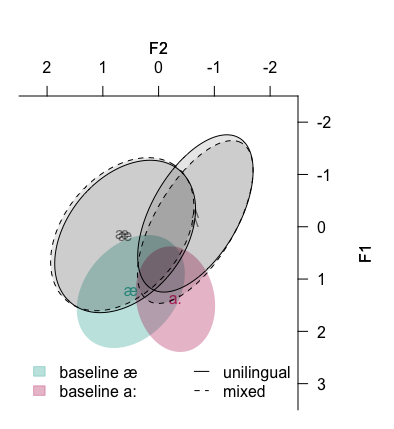
\includegraphics[scale=0.8]{vowels_e_b_final}
	\caption{Vowel categories in unilinual English (solid lines), mixed condition (dotted lines), and baseline Bengali (colored ellipses)}
	\label{vowels_e_b}
\end{figure}

Our third research question concerned the experimental paradigms. \cite{olson2013bilingual} proposes that in both scripted and spontaneous code-switching paradigms, ``discursive properties may partially drive the production of code-switches, masking underlying effects of interaction", and thus proposes cued picture-naming as a preferable alternative. This calls to question the comparability of results between studies using these different paradigms. We tested this by comparing productions of the same items from the same group of participants in a scripted CS paradigm and a cued picture-naming paradigm. We found no significant interaction of Task either with Context, or with the Vowel*Context interaction, suggesting that the extent of phonetic transfer was not affected by the paradigm. 
There are at least two plausible reasons for this-- (i) it is possible that the planning effects of CS do not translate to an increase/decrease in observable transfer at all. This would mean that the hyperarticulation seen, for example, in \cite{muldner2019phonetics} is better interpreted as resulting from some other aspect of the experimental setup, rather than the act of code-switching itself. While planning could additionally affect the words preceding the switch, the effects on the switched token itself do not change. (ii) Our study used a frame sentence to induce code switching, and not all the items led to pragmatically meaningful sentences. Thus, another possible explanation is that the discursive effects discussed by \cite{olson2013bilingual} are triggered by more naturalistic paradigms where attention to meaning and interlocutor are important. More within-study comparisons with less structured paradigms, and spontaneous code-switching data, can shed light on this. The results of the present study suggest that for the purposes of observing dynamic phonetic transfer, elicitation through cued-picture-naming vs (controlled) code-switching does not seem to significantly alter the behavior under study, and thus the choice of paradigm can be based on other considerations. Moreover, this suggests that (all else being equal) the results from such studies can be compared directly. 

Paradigm did affect vowel quality, but this applied uniformly across experimental conditions---all vowels were more backed and lowered in the code-switching task. Given that at least for F1, the effect is limited to the early stages of articulating the vowel, it is plausible that this lowering is an artifact of the particular stimuli used here---resulting from some corarticulatory effect that was absent in the picture-naming task. While this is intriguing, it is beyond the scope of the present study.  


Mixed language processing temporarily increases cross-language phonetic transfer, causing an L2 vowel to converge towards a related L1 category. The extent and direction of such shift is mediated by language-specific distribution of sound categories. In a controlled experimental setup to study transfer effects, the postulated discursive factors in a code-switching paradigm does not change the patterns of observed transfer relative to a cued picture-naming paradigm.



%\printbibliography %for use with biblatex; comment out if you use natbib
\bibliography{references} %for use with natbib; comment out if you use biblatex, and change 'sample' by the name of your bib-file


\end{document}
%%% Local Variables:
%%% mode: latex
%%% TeX-master: t
%%% TeX-engine: luatex
%%% End:
